In this section, we survey the present status of LQCD calculations of the nucleon axial form factor after providing a high-level introduction to LQCD.


\bigskip\noindent
\textbf{\large \color{red}Alternative Introduction to Lattice QCD:}

\noindent
Lattice QCD has been and remains one of the major uses of the worlds leadership computing facilities.
There is an extensive literature on LQCD covering the broad range of technical and formal aspects that are necessary to cary out state of the art calculations, for which we can not do justice in this review.
Rather, for an in depth introduction to lattice QCD, we refer readers to the text books~\cite{Smit:2002ug,DeGrand:2006zz,Gattringer:2010zz} and in this review, we provide a high-level summary of general issues that must be addressed as well as issues specific to LQCD calculations of nucleon matrix elements and form factors.


% ------------------------------------------------------------------------------
% LQCD Intro
\subsection{Lattice QCD\label{sec:lqcd_intro}}
LQCD has been and remains one of the major uses of the world's leadership computing facilities.
There is an extensive literature on LQCD covering the broad range of technical and formal aspects that are necessary to cary out state of the art calculations, for which we can not do justice in this review.
Rather, for an in depth introduction to LQCD, we refer readers to the text books~\cite{Smit:2002ug,DeGrand:2006zz,Gattringer:2010zz} and in this review, we provide a high-level summary of general issues that must be addressed as well as issues specific to LQCD calculations of nucleon matrix elements and form factors.
These issues are also discussed in detail in the bi-annual FLAG Reviews, see for example the most recent one~\cite{Aoki:2021kgd}.%
%-------------------------------------------------------------------------------
\begin{marginnote}
\entry{FLAG}{Flavour Lattice Averaging Group}
\end{marginnote}


The promise of LQCD is to provide predictions of low-energy hadronic and nuclear quantities with fully quantified theoretical uncertainties rooted in the Standard Model.
In order to deliver upon this promise, there are several sources of systematic uncertainty which must be quantified.
For all LQCD calculations, these include extrapolations to the continuum and infinite volume limits as well as an extrapolation or interpolation to the physical quark mass limit.
For the continuum extrapolation, at least three values of the lattice spacing, $a$, of $\mathrm{O}(a\lesssim0.12\textrm{ fm})$ are required to ascertain if the leading discretization corrections are sufficient or not to describe the observed scaling violations (do all three results lie on a straight line or can one detect higher-order curvature?).
For the finite volume effects, a rule of thumb has been established from experience, that one requires calculations with $m_\pi L \gtrsim4$ (where $L$ is the spatial extent of the lattice volume) in order to keep these finite size corrections at the level of $\lesssim1-2\%$ and at least qualitatively described by the leading analytic formulae.%
\begin{marginnote}
    \entry{$\chi$PT}{Chiral Perturbation Theory: the low-energy effective field theory of QCD}
\end{marginnote}%
For the light-quark mass dependence, $\chi$PT may be able to guide the extrapolations.
However, for the nucleon, the convergence of $\chi$PT is not yet established, even at the physical pion mass with evidence of lack of convergence for the nucleon mass and $g_{\mathrm{A}}$~\cite{Chang:2018uxx,Walker-Loud:2019cif}.
As we will discuss more in Section~\ref{sec:calc_anatomy}, for properties of nucleons, there are two additional significant sources of systematic uncertainty which are the exponentially%
\begin{marginnote}
    \entry{S/N}{Signal-to-noise}
\end{marginnote}%
degrading S/N problem for nucleons and excited state contamination.



%-------------------------------------------------------------------------------
% LQCD Intro
\subsection{LQCD: A High Level Summary}
The QCD path integral is quadratic in the quark fields allowing for an analytic integration over the fermionic fields such that in Euclidean space, one has the gluonic integral
\begin{equation}\label{eq:Z_QCD}
Z_{\mathrm{QCD}} = \int D U\, {\rm Det}[\Dslash(U) + m_q]\, e^{-S_{\mathrm{G}}(U)},
\end{equation}
with gluon action $S_{\mathrm{G}}(U)$ and the determinant of the quark operator ${\rm Det}[\Dslash(U) + m_q]$, for each flavor of quark simulated.
Even at finite lattice spacing and volume, the multi-dimensional integral is vastly too large to perform.
However, in Euclidean space, the fermion determinant is real and positive for zero chemical potential, as well as $S_{\mathrm{G}}$, and so the integral can be approximated with an HMC algorithm~\cite{Duane:1987de} using the factor ${\rm Det}[\Dslash(U) + m_q]\, e^{-S_{\mathrm{G}}(U)}$ as the importance sampling weight.%
%-------------------------------------------------------------------------------
\begin{marginnote}
\entry{HMC}{Hybrid Monte Carlo}
\entry{Configurations}{Samples of the gluon field}
\entry{Ensemble}{A set of configurations all generated with the same bare QCD parameters}
\end{marginnote}%
%-------------------------------------------------------------------------------
In this way, a large number of configurations of gauge fields can be generated, providing estimates of correlation functions
\begin{equation}
\langle O \rangle = \frac{1}{N_{\rm cfg}}\sum_{i=1}^{N_{\rm cfg}} O[U_i]
    +\mathrm{O}\left(\frac{1}{\sqrt{N_{\rm cfg}}} \right)\, ,
\end{equation}
where $O[U_i]$ is the correlation function evaluated on configuration $i$.
The most expensive part of generating the configurations is evaluating the fermion determinant for the light and strange quarks.
This is done with the use of pseudo-fermions (bosonic fields, $\phi$)
\begin{equation}
Z_\psi = \int D\bar{\psi}D\psi\, e^{-\bar{\psi}[\Dslashe[U]+m_q]\psi}
    = {\rm Det}[\Dslash(U) + m_q]
    = \int D\phi^\dagger D\phi\, e^{-\phi^\dagger \frac{1}{\Dslashe[U]+m_q} \phi}
\end{equation}
for which the bilinear operator is the inverse of the Dirac operator, which is a large, sparse matrix.
Most of the algorithmic development for accelerating LQCD has gone into efficiently solving these large sparse matrices with large condition numbers.  In particular, this is a problem very well suited for GPUs
for which we have an advanced library, QUDA~\cite{Clark:2009wm,Babich:2011np}, developed for the international community.%
%-------------------------------------------------------------------------------
\begin{marginnote}
\entry{GPU}{Graphical Processing Unit}
\end{marginnote}%
%-------------------------------------------------------------------------------


There are many valid choices one can make in constructing the discretized lattice action, provided continuum QCD is recovered as $a\rightarrow0$.
This is known as the universality of the continuum limit, with each choice only varying at finite lattice spacing.
Deviations from QCD, which arise at finite $a$, are often called \textit{discretization corrections} or \textit{scaling violations}.
That all lattice actions reduce to QCD as $a\rightarrow0$ is known as the universality of the continuum limit.  It is a property which can be proved in perturbation theory but must be established numerically given the non-perturbative nature of QCD.  For sufficiently small lattice spacings, one can use EFT to construct a continuum theory that encodes the discretization effects in a tower of higher dimensional operators. This is known as the Symanzik EFT for lattice actions~\cite{Symanzik:1983dc,Symanzik:1983gh}.%
%-------------------------------------------------------------------------------
\begin{marginnote}
\entry{Universality}{All valid choices of discretized QCD become QCD as $a\rightarrow0$}
\entry{EFT}{Effective field theory}
\end{marginnote}%
%-------------------------------------------------------------------------------
One interesting example involves the violation of Lorentz symmetry at finite lattice spacing: in the Symanzik EFT, the operators which encode this Lorentz violation scale as $a^2$ with respect to the operators which survive the continuum limit, and thus, Lorentz symmetry is an accidental symmetry of the continuum limit.  It is not respected at any finite lattice spacing, but the measurable consequences vanish as $a^2$ for sufficiently small lattice spacing.

For example, consider the discretized gluon action.
The link fields are Wilson lines
\begin{equation}
U_\mu(x) = \exp\left\{i a\int_0^1 dt A_\mu(x +(1-t)a\hat{\mu}) \right\}
    \approx \exp\left\{i a \bar{A}_\mu(x) \right\}\, .
\end{equation}
The gluon field $A_\mu(x)$ can be approximated as constant over the interval $[x, x+a\hat{\mu}]$, as expressed by $\bar{A}_\mu(x)$, with $a$ being the lattice spacing.
This parameterization allows for the construction of a discretized theory which preserves gauge-invariance~\cite{Wilson:1974sk}, a key property of gauge theories.
In the continuum, the gluon action-density is given by the product of field strength tensors, which are gauge-covariant curls of the gauge potential.
%\begin{align}
%&\mathcal{L}_{\mathrm{G}} = \frac{1}{2g^2}\textrm{Tr}\left[G_{\mu\nu} G_{\mu\nu}\right]\, &
%&G_{\mu\nu} = \partial_\mu A_\nu - \partial_\nu A_\mu +i [A_\mu, A_\nu]\, ,&
%\end{align}
%where $g$ is the gauge coupling.
When constructing the discretized gluon-action, it is therefore natural to use objects which encode this curl of the gauge potential.  The simplest such object is referred to as a ``plaquette'' and given by
\begin{equation}
\hspace{-1.25in}\Umunu \hspace{-0.65in}
    =U_{\mu\nu}(x)
    =U_\mu(x)U_\nu(x+a\hat{\mu}) U^\dagger_\mu(x+a\hat{\nu}) U^\dagger_\nu(x)\, .
\end{equation}
For small lattice spacing $a$, this Wilson gauge-action reduces to the continuum action plus irrelevant (higher dimensional) operators which vanish in the continuum limit
\begin{align}\label{eq:gluon_action}
S_{\mathrm{G}}(U) &= \beta \sum_{n=x/a} \sum_{\mu<\nu}
    \textrm{Re}\left[ 1 - \frac{1}{N_c} \textrm{Tr} \left[U_{\mu\nu}(n) \right]\right]
\nonumber\\&=
    \frac{\beta}{2N_c}
    a^4 \sum_{n=x/a,\mu,\nu}
    \left[
        \frac{1}{2} \textrm{Tr} \left[ G_{\mu\nu}(n)G_{\mu\nu}(n)\right]
        +\mathrm{O}(a^2)
    \right]\, ,
    & \rightarrow \beta = \frac{2N_c}{g^2}\, .
\end{align}
The continuum limit, which is the asymptotically large $Q^2$ region, is therefore approached as $\beta\rightarrow\infty$ where $g(Q^2)\rightarrow 0$.


The inclusion of quark fields adds more variety of lattice actions, each with their own benefits and drawbacks.
There are four commonly used fermion discretization schemes which are known as staggered fermions~\cite{Kogut:1974ag,Banks:1975gq,Banks:1976ia,Susskind:1976jm}, clover-Wilson fermions~\cite{Sheikholeslami:1985ij}, twisted mass fermions~\cite{Frezzotti:2000nk} and DWF~\cite{Kaplan:1992bt,Shamir:1993zy,Furman:1994ky}.%
%-------------------------------------------------------------------------------
\begin{marginnote}
\entry{DWF}{Domain Wall Fermions}
\end{marginnote}%
%-------------------------------------------------------------------------------
In this review, we comment that:
\begin{itemize}[leftmargin=*]
\item Staggered fermions are the least expensive numerically to simulate, have leading scaling violations of $\mathrm{O}(a^2)$, and they have a remnant chiral symmetry protecting the quark mass from additive mass renormalization.  However, they split the four components of the fermion spinor onto different components of a local hypercube, mixing the Dirac algebra with spacetime translations.  This significantly complicates their use for baryons~\cite{Golterman:1984dn,Bailey:2006zn,Lin:2019pia}.

\item Clover-Wilson fermions are the most commonly used discretization scheme given their theoretical simplicity and preservation of all symmetries except chiral symmetry.  The explicit breaking of chiral symmetry with the Wilson operator means the light quark masses must be finely tuned against ultra-violet chiral symmetry breaking that scales as $1/a$, after which there remain residual $\mathrm{O}(a)$ chiral symmetry breaking effects.  It is well known, albeit laborious, how to non-perturbatively remove these leading $\mathrm{O}(a)$ scaling violations~\cite{Luscher:1996sc,Luscher:1996ug,Luscher:1996jn,Capitani:1998mq}, which must be done for both the action as well as matrix elements.

\item Twisted mass fermions are a variant of Wilson fermions that exploits the approximate $SU(2)$ chiral symmetry of QCD to introduce a twisted quark mass term, $i\mu\g_5 \tau_3$.  At maximal twist, the bare quark mass is cancelled by the $1/a$ additive quark mass, leaving $\mu$ as the only contribution through $\mathrm{O}(a)$ to the physical quark mass.  Indeed, all observables are automatically $\mathrm{O}(a)$ improved at maximal twist~\cite{Frezzotti:2003ni}.
However, twisted mass fermions break isospin symmetry at finite lattice spacing, causing some complications now that LQCD results are precise enough to require isospin breaking corrections from $m_d-m_u$ and%
\begin{marginnote}
\entry{QED}{Quantum electro-dynamics}
\end{marginnote}%
QED to be compared with experiment.

\item The fourth most common discretization are DWF, which introduce a fifth dimension to the theory with unit links (the gluons are not dynamic in the fifth dimension) with the left and right handed fermions bound to opposite sides of the fifth dimension of size $L_5$.  The overlap of these left and right modes gives rise to an explicit chiral symmetry breaking that is exponentially suppressed by the extent of the fifth dimension.  For sufficiently small chiral symmetry breaking (large $L_5$), DWF are also automatically $\mathrm{O}(a)$ improved.
While very desirable, DWF are numerically more expensive to simulate, both because of the extra fifth dimension and also because the algorithmic speed up offered by multi-grid, which works tremendously for clover-Wilson fermions on GPUs~\cite{Clark:2016rdz}, is not yet flushed out for DWF~\cite{Boyle:2014rwa,Cohen:2011ivh,Yamaguchi:2016kop,Brower:2020xmc,Boyle:2021wcf}.

\item A final common variant of action is one in which the fermion discretization used in the generation of the gauge fields (the sea quarks) and the action used when generating quark propagators (the valence quarks) are different: this is known as a \textit{mixed action}~\cite{Renner:2004ck}.
The most common reason to use such an action is to take advantage of numerically less expensive methods to generate the configurations while retaining good chiral symmetry properties of the valence quarks, which is known to suppress chiral symmetry breaking effects from the sea-quarks~\cite{Bar:2002nr,Bar:2005tu,Tiburzi:2005is,Chen:2007ug}.

\end{itemize}
As mentioned above, a key assumption of LQCD is that all varieties of lattice action, for sufficiently small lattice spacing, are approximated by continuum QCD plus irrelevant operators whose contributions vanish in the continuum limit.
It is important for the field to test this assumption of universality by computing the same quantities with a variety of lattice actions, both at the level of gluons as well as the fermions, in order to gain confidence in the results that are extrapolated to the physical point.


% ------------------------------------------------------------------------------
% anatomy of LQCD calculation
\subsection{Anatomy of LQCD Calculations of Nucleon Form Factors\label{sec:calc_anatomy}}


% ------------------------------------------------------------------------------
% LQCD PCAC
\subsection{Role of PCAC in lattice QCD results of $F_A(Q^2)$\label{sec:lqcd_pcac}}
%\cw{Some repetition between this paragraph and Section 2.}
%Computations of the nucleon axial charge have long been considered
% a vital benchmark for nucleon physics with LQCD.
%This quantity has been precisely measured with experiments probing neutron beta decay,
% characterized by a weak decay with a low momentum transfer.
%Historically, lattice calculations of the axial charge have obtained values
% that were $O(10\%)$ too low, despite significant investments of effort.
%This has been the subject of some controversy,
% with more and more sophisticated calculations to scrutinize lattice systematics.
%Over time, contamination from excited states was identified as
% an important contributing factor to the systematic deviation.
%Many collaborations have opted for high-statistics computations
% to reduce the statistical uncertainty at late times and permit
% multi-exponential fits to the time dependence of the correlation functions.
%As time progressed, LQCD results moved closer to the experimental value,
% and now modern calculations are in agreement with experiment
% at the 1\% level~\cite{Kronfeld:2019nfb}.
%\textcolor{red}{[more citations]}

\new{$F_{\rm A}(Q^2)$ can be isolated in LQCD calculations with particular kinematic choices that are not contaminated by the induced pseudoscalar form factor, see for example Ref.~\cite{Gupta:2017dwj}.
Given the challenges in identifying all the sources of systematic uncertainty in the calculation of $g_A$, particularly the excited state contamination, it is prudent to perform cross checks of observables to test for consistency of the results.}
%
%Modern efforts to compute nucleon matrix elements now target the nucleon
% axial form factor with its four-momentum transfer dependence.
%Given how difficult the axial charge has been to accurately determine,
% cross checks of observables computed with lattice QCD are vital
% for testing consistency of the results.
%To check the accuracy of LQCD calculations targeting the axial form factor,
% the validity of the PCAC relation,
The validity of the PCAC relation,
\begin{align}
 \partial^\mu A^{a}_{\mu}(x) = 2 m_q P^{a}(x),
 \label{eq:pcac}
\end{align}
\new{provides a complex consistency check.}
% has been scrutinized with lattice data.
%is the most reasonable choice for checking consistency.
Here, $A^{a}_\mu$ and $P^{a}$ are the axial and pseudoscalar currents,
 respectively, and $m_q$ is the light quark mass.
The PCAC relation is an exact symmetry in the continuum limit.
The generalization of this relation to the nucleon form factors
 yields the GGT%
 \begin{marginnote}
 \entry{GGT}{Generalized Goldberger-Triemann relation (Equation~\ref{eq:ggt})}
 \end{marginnote}%
 relation,
\begin{align}
 2 m_{\mathrm{N}} F_{\mathrm{A}}(Q^2) -\frac{Q^2}{2m_{\mathrm{N}}} \widetilde{F}_{\mathrm{P}}(Q^2) = 2 m_q F_{\mathrm{P}}(Q^2),
 \label{eq:ggt}
\end{align}
 which provides orthogonal checks of individual matrix elements
 for the axial and pseudoscalar currents.
The axial, induced pseudoscalar, and pseudoscalar form factors of the nucleon
 ($F_{\mathrm{A}}$, $\widetilde{F}_{\mathrm{P}}$, and $F_{\mathrm{P}}$, respectively) appear in this expression,
 and $m_{\mathrm{N}}$ is the nucleon mass.
The PPD ansatz, \new{which is only approximate even in the continuum limit,}% is also studied,%
\begin{marginnote}
 \entry{PPD}{Pion pole dominance}
 \end{marginnote}%
\begin{align}
 \widetilde{F}^{\rm PPD}_{\mathrm{P}}(Q^2) = \frac{4m_{\mathrm{N}}^2}{Q^2+m_\pi^2} F_{\mathrm{A}}(Q^2),
 \label{eq:ppd}
\end{align}
% which is only approximate even in the continuum and
is obtained
 by carefully considering the leading asymptotic behavior of the
 form factors in the double limit $Q^2\to0$ and $m_q\to0$~\cite{Sasaki:2007gw}.
%In this expression, $m_\pi$ is the pion mass.

Initial calculations targeting the axial form factor verified the PCAC relation
 for the full correlation functions but found significant \emph{apparent} violations
 of GGT~\cite{Ishikawa:2018rew,Gupta:2017dwj,Bali:2018qus}. The resolution of this apparent violation
 is now informed by baryon $\chi$PT, which suggests that chiral
 and excited state corrections to the spatial axial, temporal axial, and induced pseudoscalar
 are functionally different and not properly removed.
The axial contributions are largely dominated by loop-level $N\pi$ excited states
 with a highly suppressed tree-level correction.
The correction to the axial current is nearly independent of $Q^2$.
On the other hand, corrections to the induced pseudoscalar are
 driven by the tree-level correction and has
 a strong $Q^2$ dependence~\cite{Bar:2018xyi}, with the largest correction at low $Q^2$.
The $N\pi$ loop contribution in the induced pseudoscalar is highly suppressed by
 an approximate cancellation.
The contamination to the pseudoscalar current is redundant with the
 axial and induced pseudoscalar chiral corrections and can be obtained
 by application of the PCAC relation.

Scrutiny of the LQCD data has demonstrated many of the features
 that were expected from chiral perturbation theory.
The primary excited state contaminations to the axial form factor matrix elements
 were shown to be driven by two specific $N\pi$ states,
 characterized by a transition through an axial current
 of the nucleon state to an $N\pi$ excited state or vise versa~\cite{Jang:2019vkm}.
In the language of $\chi$PT, these states contribute to tree-level nucleon-pion graphs with fixed relative momentum~\cite{Bar:2018xyi}.
These $N\pi$ states were initially expected to be negligible due to a volume suppression
 of the state overlap, which makes them invisible to the two-point functions~\cite{Bar:2016uoj}.
However, the three-point axial matrix element enhances these contributions relative
 to the ground state nucleon matrix element, which is enough to overcome the volume suppression.
As a consequence, analyses that fix the spectrum using the two-point functions alone
 will often miss the important $N\pi$ contamination to the
 axial matrix element~\cite{Jang:2019vkm,He:2021yvm}.

The lattice data also showed deviations as large as $40\%$ from the PPD
 ansatz at low $Q^2$, where it was expected to
 work best~\cite{Bali:2014nma,Gupta:2017dwj}.
Each $Q^2$ prefered dominant $N\pi$ states with different energies,
 which when neglected across the full range of momentum transfers
 produced a $Q^2$-dependent discrepancy in excess of the $Q^2$ behavior
 expected from the GGT and PPD relations.
Fits to the three-point functions that allow for the possibility of
 nonnegligible $N\pi$ states are able to constrain the effects of these states,
 removing the contamination and thereby restoring the PPD relation.

\new{
Nucleon matrix elements of the temporal axial current have the largest visible excited state contamination~\cite{Jang:2019vkm,RQCD:2019jai} which can be at least qualitatively understood with $\chi$PT~\cite{Bar:2018xyi}.
This has led to new analysis strategies that more carefully deal with the $N\pi$ excited state with pion-pole contributions, yielding minimal violations of PCAC that include such matrix elements, and a better understanding of the impact of these excited states on different matrix elements that are sensitive to either $F_{\rm A}(Q^2)$ or $\tilde{F}_{\rm P}(Q^2)$.}

\new{
While these results are very encouraging, they are not conclusive in the sense that they require us to impose our theoretical prior on the analysis, rather than the results naturally ``falling out'' from the numerical analysis.
In order to achieve this more stringent validation, the calculations would have to generally be performed at larger source-sink separation times where the correlation functions are all saturated by the ground state, but the noise is exponentially larger.
Given the extreme cost of such a strategy, a better solution would be to implement a variational method that allows for the use of multi-hadron operators that can explicitly remove the $N\pi$ excited states through a diagonalization of the correlation functions~\cite{Blossier:2009kd}.  We will return to this point in Section~\ref{sec:future}.}


% ------------------------------------------------------------------------------
% LQCD results
\subsection{Survey of lattice QCD results of $F_A(Q^2)$\label{sec:lqcd_results}}

%\new{
%The cost of performing a calculation of the nucleon axial form factor,
% both in terms of computation time and human time for analysis,
% is significantly more than what is required for a computation the axial charge.
%Despite the active efforts collaborations have had in computing the axial form factor,
% the costs have been a limiting factor in the availability of results.
%}

\asm{moved up}
Though the axial \new{charge and} radius are useful for connecting with low-energy applications,
 such as pion electroproduction and neutron decay applications,
 the needs of neutrino physics in the GeV-scale energy range depend
 on the full momentum transfer dependence of the form factor.
The main deliverables from lattice QCD calculations of the axial form factor
 are the axial and induced pseudoscalar form factors taken in the continuum-chiral
 and infinite volume limits, complete with a set of parameterization coefficients
 and covariance matrix.
This is especially true considering the agreement between LQCD and experiment
 for the axial radius taken together with the observation that
 LQCD prefers a slower form factor fall off than experiment,
 \new{plotted in Figure~\ref{fig:gaq2_overlay}}.
If the axial radius were the only parameter determining the form factor $Q^2$ dependence,
 then these two observations are incompatible.
Though the form factor shape, especially when allowed to explore its full uncertainty,
 is decidedly \emph{not} a dipole shape, the central value curve determined
 from experiment appears to follow a dipole-like shape.
Restricting to dipole shape only, agreement with the axial radius at $Q^2=0$
 would mean the axial form factor should agree over the entire relevant $Q^2$ range,
 a statement that is not supported by the LQCD data.
\new{
There is no reason to expect nature to prefer a dipole-like parameterization ---
 the experimental preference toward a dipole-like parameterization is based on
 a few datasets from the early 1980s~\cite{ANL_Barish_1977, BNL_Baker_1981, Kitagaki:1983px}
 with $O(10^3)$ events at most,
 on deuterium targets with nuclear corrections that are likely underestimated~\cite{Meyer:2016oeg}.
In addition, the dipole parameterization violates
 unitarity constraints imposed by QCD~\cite{Bhattacharya:2011ah}
 and is primarily motivated by its asymptotic behavior at high-$Q^2$,
 a regime well outside of the kinematic range probed by neutrino scattering experiments.
}
\done{I wonder if it's useful to highlight that the experimental data here is a small number of events from two old experiments? Whenever anything is contrasted with ``experiment'' I worry that it may not be clear to readers that the experiment is crap...}

\textcolor{red}{[description of summary plot]}
\new{
Figure~\ref{fig:gaq2_overlay} shows the status of existing calculations of
 the nucleon axial form factor from lattice QCD,
 compared to the axial form factor obtained from neutrino scattering
 with deuterium in Ref.~\cite{Meyer:2016oeg}.
The RQCD~\cite{RQCD:2019jai} and NME~\cite{Park:2021ypf} collaborations
 have the most mature analyses with several ensembles that probe a range of
 systematic effects.
These computations each have their own methods for addressing the
 excited state contaminations discussed in Sec.~\ref{sec:lqcd_pcac},
 which successfully restore the GGT relation.
RQCD modify the parameterization used to fit the correlation function
 to better constrain the expected shape of excited state contamination from the $N\pi$ states.
NME test a variety of Bayesian fits to constrain the excited state contributions,
 where their preferred fit enforces a tight prior on the nucleon-pion state
 at the energy expected from a naive dispersion relation.
Because these two results are based on several ensembles,
 their fits are parameterized and plotted as bands rather than as scatter points
 to distinguish them from estimates on single ensembles.
}

\begin{figure}[hbt!]
\centering
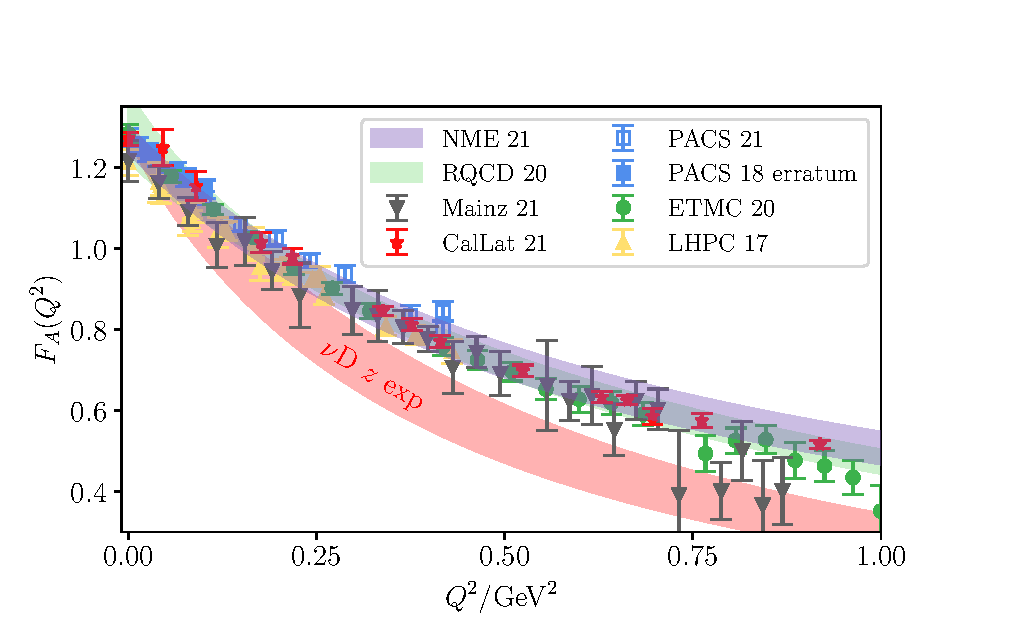
\includegraphics[width=0.5\textwidth]{plots/gaq2-overlay-standalone.pdf}
\vspace{10pt}
\caption{
Published results for the axial form factor obtained from lattice QCD,
 compared with the deuterium extraction from Ref.~\cite{Meyer:2016oeg}.
Collaborations that have obtained their results from only a single ensemble
 are plotted as scatter points.
These single-ensemble results will have small but unknown corrections due to chiral, continuum,
 and finite volume systematic shifts.
The NME~\cite{Park:2021ypf} and RQCD~\cite{RQCD:2019jai}
 results are both obtained from fits to several ensembles.
The RQCD perform the full chiral-continuum and finite volume extrapolations to the data,
 fitting to each of the form factors independently for each ensemble but providing
 the constraint that the form factors must satisfy the GGT relation in the continuum.
The NME collaboration also performed a chiral-continuum and finite volume extrapolation
 on their data, but found significantly larger uncertainties and so their result
 is obtained from an average of the results on their five largest volume ensembles.
As a rough estimate, NME claims that the uncertainties are at least a factor of 5 larger
 if the fits are relaxed to allow the results to change with pion mass or lattice spacing.
 \cw{Why are there two PACS 21 datapoints on top of each other at ~0.4 GeV$^2$}}
 \asm{Two different ways of constructing momentum vectors of magnitude 3:
 (2,2,1) and (3,0,0)}
\label{fig:gaq2_overlay}
\end{figure}

\asm{Describe callat result}
\new{
The ETMC~\cite{Alexandrou:2020okk}, LHPC~\cite{Hasan:2017wwt},
 PACS~\cite{Ishikawa:2018rew,Shintani:2018ozy,Ishikawa:2021eut}, and CalLat~\cite{Meyer:2021vfq}
 results have just a few ensembles, so scatter points obtained from fitting
 are shown rather than the form factor parameterization to distinguish
 them from extrapolated results.
Though these results are expected to be close to the physical point results,
 they will have unquantified systematic shifts.
The ETMC has three ensembles, two of which have only 2 flavors of sea quarks
 and will be subject to systematics from neglecting sea effects from strange quarks.
The remaining ETMC ensemble is a 2+1+1 flavor ensemble at physical pion mass,
 which is shown in Fig.~\ref{fig:gaq2_overlay}.
The PACS results are on two different ensembles with physical pion mass,
 with volumes of $(5.5~{\rm fm})^3$ and $(10.8~{\rm fm})^3$
The Mainz collaboration has an ongoing calculation in proceedings on 12 ensembles,
 including an ensemble at \new{the} physical pion mass
 and a chiral-continuum and infinite volume extrapolation~\cite{Djukanovic:2021yqg}.
The results from their two-state fit to the E250 physical pion mass ensemble
 are plotted with the other results.
}

\new{
The published results use different lattice actions for the simulations ---
 NME~\cite{Park:2021ypf}, RQCD~\cite{RQCD:2019jai}, Mainz~\cite{Djukanovic:2021yqg},
 LHPC~\cite{Hasan:2017wwt}, and PACS~\cite{Ishikawa:2018rew,Shintani:2018ozy,Ishikawa:2021eut}
 use different sets of ensembles of $2+1$ flavor $O(a)$-improved Wilson clover fermions,
 ETMC~\cite{Alexandrou:2020okk} use twisted mass fermions with a clover term,
 and CalLat~\cite{Meyer:2021vfq} uses a mixed-action setup with M\"obius domain wall quarks
 on HISQ~\cite{MILC:2012znn}%
 \begin{marginnote}
  \entry{HISQ}{Highly-improved staggered quarks}
 \end{marginnote}%
 gauge configurations.
The general agreement between calculations with different actions tests
 the universality of fermion actions.
No obvious tensions are seen,
 leading to the conclusion that there are no significant scaling violations
 in the data due to nonzero lattice spacing.
The restriction to finite volume has also been probed to some extent by
 the PACS collaboration results, %~\cite{Ishikawa:2018rew,Shintani:2018ozy}
 again with no obvious deviations from the results of other collaborations.
}

\asm{moved up}
The excellent agreement of the axial form factor data and parameterizations
 for all of the LQCD simulations provides credibility to the claims
 made by the lattice collaborations, in particular the slow falloff with $Q^2$.
Despite the apparent violations of GGT in the low-$Q^2$ region,
 the high-$Q^2$ region seems to be in better control and not as sensitive to
 the same excited state contamination.
The high-$Q^2$ agreement is reflected by the restoration of the GGT relation at large $Q^2$,
 which is generally the case even for computations that have difficulty satisfying
 the GGT relation at low $Q^2$.
%This is expected based on the approximation that the
% two dominant $N\pi$ excited states are the only excited state contaminations,
% which indicates a mass gap that grows with $Q^2$ leading to a larger suppression.
%\textcolor{red}{[ but the $N\pi$ contribution from XPT is constant with $Q^2$,
% so something isn't right ]}
\new{These claims could be spoiled by systematic effects
 that are common to all of the calculations,
 and excited state contaminations from $N\pi$ states in
 the axial form factor remain as a dominant concern.
While estimates of excited states using methods that are currently employed
 by lattice calculations have helped to clarify the situation,
 modern calculations with $N\pi$-like interpolating operators
 are needed to definitively quantify the excited state contaminations over all $Q^2$.}
%Modern calculations with $N\pi$-like interpolating operators should be able
% to isolate these remnant excited state contributions in order to make
% concrete statements about the relative size of the $N\pi$ contamination over $Q^2$.
\new{If a dedicated calculation can demonstrate that the
 excited states are controlled well by the methods presently in use},
 then worries about the contamination should be more or less resolved.

Another concern is that the magnitude of $Q^2$ may adversely affect
 the convergence of the chiral expansion at large $Q^2$,
 limiting the ability to extrapolate lattice QCD results to the physical point.
Even for low and moderate values of momentum transfer,
 a large expansion order would be needed to constrain the form factor
 dependence on the relevant low energy constants,
 limiting the predictability of the theory.
There is some hope that expanding in terms of the $z$ expansion parameter $z$
 may alleviate some of these concerns by building in correlations between
 low and high orders of $Q^2$ that are expected from analyticity.
This will be discussed in more detail in Section~\ref{sec:z_continuum},
 where the relationship between $Q^2$ and $z$ will be analyzed in more detail.

%\textcolor{red}{[NME]}
%\textcolor{red}{[RQCD]}
%
%\textcolor{red}{[ETMC]}
%The ETMC calculation~\cite{Alexandrou:2020okk} of the axial form factor
% is performed on three ensembles with twisted mass fermions all at physical pion mass.
%Two of these ensembles include only light quarks in the sea,
% leading to unquantifiable systematic corrections from
% neglecting the effects of strange quarks.
%However, these two two-flavor ensembles permit an explicit test of finite-volume corrections,
% demonstrating a lack of dependence on the volume in the range of typical lattice computations.
%The remaining ensemble has four flavors of sea quarks and thus is not subject
% to the same criticism of neglecting the strange quarks.
%Despite the agreement with the trend of axial form factor results from other collaborations,
% the results from this computation do not satisfy the PPD and GGT relations,
% suggesting remnant excited state contamination.
%
%\textcolor{red}{[PACS]}
%The PACS collaboration has focused on computing the axial form factor
% on large ensembles with Wilson clover fermions at
% physical pion mass~\cite{Ishikawa:2018rew,Shintani:2018ozy}.
%The ensemble used in this analysis has a volume of $(10.8~{\rm fm})^3$,
% considerably larger than ensembles used by other collaborations.
%The large volume reduces the minimum $Q^2$ that can be probed
% with the discrete lattice momenta but forces the need for many units of momenta
% to access the same kinematic range as other computations.
%They compare this ensemble to a computation of the axial radius using
% the traditional method compared with derivatives obtained from
% moments of the correlators~\cite{Aglietti:1994nx},
% on a $(5.5~{\rm fm})^3$ volume ensemble, finding agreement between the results of each.
%Results on both ensembles are about $1\sigma$ small compared to the axial radius
% from the average from experimental sources in Ref.~\cite{Hill:2017wgb}.
%Like the ETMC results, the PACS calculation does not satisfy the PPD and GGT relations.
%
%\textcolor{red}{[LHPC]}
%The LHPC collaboration have an axial form factor computation on a
% single ensemble of Wilson clover fermions at physical pion mass~\cite{Hasan:2017wwt}.
%This methodology paper focuses on computing the nucleon charges
% and radii by explicitly computing derivatives of the correlation functions
% with respect to the momentum transfer.
%This method yields the axial radius directly from $Q^2=0$ data,
% which is compared to the nucleon form factor slopes and charges obtained from
% fits to data at nonzero $Q^2$ using the traditional three-point correlator methods.
%Though the results are in agreement between the two methods,
% the direct derivative proves to be noisier than the traditional method.
%With more precision, the axial radius obtained from this method,
% or constraints on the slope obtained in a similar fashion at nonzero $Q^2$,
% could provide orthogonal constraints on the form factor that could
% help pin down the axial form factor shape.

\textcolor{red}{[Other calculations]}
In addition to the aforementioned published results, \new{there are}
 a handful of recent preliminary results that deserve mention.
The LHPC~\cite{Hasan:2017wwt} and PACS~\cite{Ishikawa:2021eut} collaborations
 explore methods for directly computing the form factor values and slopes
 directly at $Q^2=0$, which offer alternative methods for constraining
 the form factor shape that could be used to complement traditional methods.
The Fermilab Lattice and MILC collaborations also have an ongoing
 computation of the axial form factor using a unitary HISQ-on-HISQ setup,
 for which a preliminary computation of the axial charge on
 a single unphysical ensemble exists~\cite{Lin:2020wko}.
Because of the choice of action, this computation has more nucleon ``tastes''
 than other efforts, which is more computationally affordable
 at the cost of a more challenging analysis.
The CalLat collaboration have a computation of the axial form factor
 using a mixed-action domain wall on HISQ setup,
 with existing data on several ensembles including multiple physical pion mass ensembles.
The fits to one physical mass ensemble from the CalLat collaboration are used
 to make statements about the \new{phenomenological} impact of the LQCD results in Sec.~\ref{sec:impact}.

\begin{itemize}
\item
\textcolor{red}{[
 temporal axial current - subject to large excited state corrections.
 ETMC claim precise, use it to constrain $N\pi$.
]}
\item
\textcolor{red}{[
 Axial form factor has different corrections than induced pseudoscalar.
 Most of $N\pi$ contamination introduced into GGT and PCAC from axial,
 enhanced by $Q^2$-dependent prefactor.
]}
\item
\textcolor{red}{[
 $g_{\mathrm{A}}(Q^2)$ parameterizations.
 $z$ expansion intro, taken from chiral section.
]}
\item
\textcolor{red}{[
 Different methods of dealing with excited states.
 FH, 3pt fits, summation, other?
]}
\end{itemize}

%Citations for $F_{\mathrm{A}}(Q^2)$ references pulled from NME21, no $g_{\mathrm{A}}$-only references:
%\begin{description}
%\item[NME 21]~\cite{Park:2021ypf}
%\item[RQCD 20]~\cite{Bali:2018qus,RQCD:2019jai} %% 63
%\item[ETMC 20]~\cite{Alexandrou:2018sjm,Alexandrou:2019brg,Alexandrou:2020okk} %% 54-56
%\item[PACS 18 (erratum)]~\cite{Ishikawa:2018rew,Shintani:2018ozy} %% 60-61 (62 proceedings)
%\item[PNDME 17]~\cite{Gupta:2017dwj,Gupta:2018qil,Jang:2019vkm,Jang:2019jkn} %% 6-9
%\item[CLS 17]~\cite{Hasan:2017wwt,Hasan:2019noy} %% LHPC? 66-67
%\end{description}
%Other axial ff effort references:
%\begin{description}
%\item[new PACS gA(Q2)]~\cite{Ishikawa:2021eut}
%\item[Mainz gA(Q2)]~\cite{Djukanovic:2021yqg}
%\item[Fermilab Lattice+MILC HISQ gA(0)]~\cite{Lin:2020wko}
%\item[CalLat gA(Q2)]~\cite{Meyer:2021vfq}
%\end{description}
%Other references:
%\begin{description}
%\item[USQCD white paper]~\cite{Kronfeld:2019nfb}
%\item[FLAG 21]~\cite{Aoki:2021kgd}
%\item[CalLat excited states $g_{\mathrm{A}}$]~\cite{He:2021yvm}
%\item[Ottnad excited states]~\cite{Ottnad:2020qbw}
%\item[Baer XPT]~\cite{Bar:2018xyi,Bar:2019igf}
%\item[Axial radius from LQCD using XPT]~\cite{Yao:2017fym}
%\end{description}


% ------------------------------------------------------------------------------
% z-expansion
\subsection{Combining the $z$-expansion with the continuum and chiral extrapolations\label{sec:z_continuum}}
LQCD results are computed at finite lattice spacing, in a finite volume and typically (for nucleons) at pion masses heavier than nature.
Even when results at the physical pion mass are available, results at heavier pion masses can help improve the overall precision of the final result, provided the extrapolation to the physical pion mass is under control.
EFT is extensively used to guide the extrapolation to the physical point.
Symanzik EFT~\cite{Symanzik:1983dc,Symanzik:1983gh} provides a continuum description of a discretized lattice action that incorporates the lattice spacing corrections through a tower of increasingly irrelevant operators.
$\chi$PT provides a description of perturbative light quark mass corrections to pions~\cite{Gasser:1984gg} and nucleons~\cite{Jenkins:1990jv,Bernard:1995dp} in a systematic expansion about the chiral limit and low momentum.
$\chi$PT can be readily extended to systematically include discretization effects by constructing the EFT from the Symanzik EFT, which includes QCD as the leading Lagrangian and discretization effects through the higher dimensional operators~\cite{Sharpe:1998xm}.
$\chi$PT can also be extended to incorporate the boundary conditions of the finite volume and describe the finite-volume corrections which scale as $m_\pi^n e^{-m_\pi L}$ for $m_\pi L \gtrsim3.5$ with the power $n$ depending upon the particular quantity of interest~\cite{Gasser:1986vb}.

While these EFTs provide a complete description of the physics at low momentum and sufficiently light pion masses, they come with LECs that capture the short-distance (L)QCD physics which are a priori unknown, given the non-perturbative nature of QCD.%
%-------------------------------------------------------------------------------
\begin{marginnote}
\entry{LEC(s)}{Low energy constant(s)}
\end{marginnote}%
%-------------------------------------------------------------------------------
The LECs describing the QCD pion mass and momentum dependence can be determined both from comparing with experimental data as well as LQCD results, while the LECs describing the discretization corrections can only be determined by comparing with LQCD results as these LECs are specific to a given lattice action.

The range of validity of $\chi$PT seems to be at best $m_\pi\lesssim300$~MeV~\cite{Beane:2004ks,Walker-Loud:2008rui} with some indications the convergence is troubled at the physical pion mass~\cite{Walker-Loud:2019cif,Drischler:2019xuo}.
The reach in $Q^2$ will likely have a similar upper bound, though this has not been examined in nearly the detail as the pion mass expansion.
For many quantities, a power series expansion in $m_\pi$ or $m_\pi^2$ may be perfectly sufficient, combined with sufficiently precise results at the physical pion mass, to guide the interpolation to the physical point, as was observed in detail for $g_A$~\cite{Chang:2018uxx}.
For example, one can consider an expansion of the form factor as a power-series in $Q^2$ with coefficients that capture the pion mass and lattice spacing dependence
\begin{align}\label{eq:F_Q_power}
F(Q^2) = \sum_{k=0} f_k(m_\pi, a) Q^{2k},
\end{align}
where these prefactors will depend upon the LECs of QCD and the discretized lattice action.
This form factor expansion will only has limited validity for $Q^2$ close to zero.
One approach to circumvent this failure mode is to appeal to the analytic structure of QCD,
performing a conformal mapping to a obtain a new small expansion parameter.
This parameterization, referred to as the $z$ expansion~\cite{Bhattacharya:2011ah},
has been utilized for decades in meson flavor physics~\cite{Okubo:1971jf}
and is a standard feature in modern LQCD calculations of meson form factors
for determining CKM matrix elements.




\iffalse
\bigskip
Lattice data are computed with nonzero lattice spacings and typically at unphysical pion masses.
To control for the effects of these systematics,
 chiral perturbation theory and a Symanzik effective theory are typically employed.
These connect the lattice results to the physical point by means
 of a perturbative expansion in parameters such as the pion mass or lattice spacing.
Powers of these expansion parameters come with some LECs
 that must be fit to the lattice data over various ensembles with different parameters.
With the LECs in hand, extrapolation to the continuum and physical pion mass
 may be completed and results obtained for QCD.

These extrapolations are known for the axial charge,
 but heavy baryon chiral expansions with $Q^2$ dependence are largely unexplored.
In their place, one might choose to instead expand the form factor as
 a power series in $Q^2$ with LEC prefactors $\ell_k$,
\begin{align}
 F(Q^2) = \sum_{k=0} \ell_k (Q^2)^k,
\end{align}
 where the $\ell_k$ have some unknown dependence on the pion mass and lattice spacing.
This form factor expansion will only has limited validity for $Q^2$ close to zero.
One approach to circumvent this failure mode is to appeal to the analytic structure of QCD and
 perform a conformal mapping to a obtain a new small expansion parameter.
This parameterization, referred to as the $z$ expansion~\cite{Bhattacharya:2011ah},
 has been utilized for decades in meson flavor physics~\cite{Okubo:1971jf}
 and is a standard feature in modern LQCD calculations of meson form factors
 for determining CKM matrix elements.
\fi



The $z$ expansion takes the four-momentum transfer squared $Q^2$
 to a small expansion parameter $z$, using the relation
\begin{align}
 z(t=-Q^2;t_0,t_c) = \frac{\sqrt{t_c-t} -\sqrt{t_c-t_0}}{ \sqrt{t_c-t} +\sqrt{t_c-t_0}}.
\end{align}
Here, $t_c$ is no larger than the particle production threshold in timelike momentum transfer
 and $t_0$ is a parameter (typically negative) that
 may be chosen to improve the series convergence.
Inverting this relation and expanding as a power series in $z$ about $Q^2=-t_0$ ($z=0$) yields
\begin{align}
x =  \frac{Q^2+t_0}{t_c-t_0} = 4 \sum_{k=1}^\infty k z^k.
 \label{eq:Q2toz}
\end{align}
Following this procedure, the dimensionful LECs that appear as prefactors for powers of $Q^2$
 are instead assembled into expressions related to the dimensionless
 coefficients of the $z$ expansion (to avoid confusion with the lattice spacing, we label the coefficients as $b_k$),
\begin{align}
 F\big(z(Q^2)\big) = \sum_{k=0}^\infty b_k z^k.
 \label{eq:zexp}
\end{align}
%
For the inverse transformation to take an expansion in $z$ to an expansion in $Q^2$,
 the expansion is again cast in terms of $x$
like in Eq.~(\ref{eq:Q2toz}).
Then the expression for $z$ at small $x$ is
\begin{align}
 (1+x)^{1/2} -1 = \frac{x}{2}
 -4\sum_{k=2}^\infty \frac{(2k-3)!}{k!(k-2)!} \biggr( -\frac{x}{4} \biggr)^{k},
 &\quad
 z = \frac{1}{x} \big( (1+x)^{1/2} -1 \big)^2,
 \label{eq:ztoQ2}
\end{align}
 which starts at $O(x)$.
For large $Q^2$, the relation is instead expanded in terms of $x^{-1}$.

A general series in $Q^2$ may therefore be converted to a double expansion in $z$ and $t_0$
 by first converting powers of $Q^2$ to those of $Q^2+t_0$ and $t_0$ using binomial theorem,
\begin{align}
 Q^{2m} &= \big( (Q^2+t_0) -t_0 \big)^m
 = (t_c-t_0)^m
 \sum_{n=0}^{m} \left( \begin{array}{c} m \\ n \end{array} \right)
 x^n
 %\biggr( \frac{Q^2+t_0}{t_c-t_0} \biggr)^n
 \biggr( \frac{-t_0}{t_c-t_0} \biggr)^{m-n}
\end{align}
 and then substituting Eq.~(\ref{eq:Q2toz}) to convert powers of $Q^2+t_0$
 into powers of $z$.
All dependence on the dimension is absorbed into powers of $t_c-t_0 \propto m_\pi^2$.
The relative weight of the expansion parameters may be adjusted by changing
 the value of $t_0$, giving some modicum of freedom over the expansion order.

The most recent multi-ensemble LQCD publications with computations
 of the axial form factor~\cite{Park:2021ypf,RQCD:2019jai}
 have treated the $z$ expansion coefficients as the relevant LECs
 and fit to these coefficients with a chiral-continuum extrapolation.
No attempt was made to connect these LECs to those obtained
 from chiral expansions with explicit $Q^2$ dependence.
Instead, observables such as $r_{\mathrm{A}}^2$ and $g_{\mathrm{A}}$
 were fit to separate chiral-continuum extrapolations.
Application of the formulae in this section exposes the relationships
 between LECs for powers of $Q^2$ to the $z$ expansion coefficients.

As a simple example, consider the $Q^4$ expansion of equation~\eqref{eq:F_Q_power} with
\begin{align}
f_0 &= c_0 + \ell_0 m_\pi^2 + d_0 a^2\, ,
\nonumber\\
f_1 &= c_1 + \ell_1 m_\pi^2 + d_1 a^2\, ,
\nonumber\\
f_2 &= c_2 + \ell_2 m_\pi^2 + d_2 a^2\, ,
\label{eq:lecampi}
\end{align}
where $c_k$, $\ell_k$ and $d_k$ are LECs describing the pion mass and lattice spacing dependence.
For the axial form factor, $c_0$ and $c_1$ are related to the axial charge and radius in the chiral limit
\begin{align}
&c_0 = \lim_{m_\pi\rightarrow0} g_A\, ,&
&c_1 = -\lim_{m_\pi\rightarrow0} \frac{g_A r_A^2}{6}\, .&
\end{align}
Then the $z$ expansion coefficients that appear in equation~(\ref{eq:zexp})
 expressed in terms of these LECs are
\newcommand{\tctza}{\ensuremath{(t_c-t_0)}}
\newcommand{\tctzb}{\ensuremath{\Big(\frac{-t_0}{t_c-t_0}\Big)}}
\begin{align}\label{eq:z_coeff_xpt}
b_0 &= f_0 +\tctza \tctzb f_1 +\tctza^2 \tctzb^2 f_2 +O\big(\tctza^3\big),
\nonumber\\
b_1 &= 4 \tctza f_1 +8 \tctza^2 \tctzb f_2 +O\big(\tctza^3\big),
\nonumber\\
b_2 &= 8 \tctza f_1 +16 \tctza^2 \Big(1 -\frac{t_0}{t_c-t_0}\Big) f_2 +O\big(\tctza^3\big).
\end{align}
Then the leading lattice spacing and pion mass dependence from
 the LECs for the $Q^2$ expansion may be made manifest
 by substituting their expresions from equation~(\ref{eq:lecampi}).
Higher-order corrections to the $\chi$PT expressions may be checked
 by peforming fits to the LECs of the $z$ expansion and comparing those
 to fits to the LECs of the $Q^2$ expansion.

When the $z$-expansion coefficients are expressed as in equation~\eqref{eq:z_coeff_xpt}, this opens the possibility of performing a simultaneous $z$-expansion fit to LQCD results of the form factors on multiple ensembles simulated at different lattice spacings, pion masses and volumes.
Similarly, the finite volume corrections can also be incorporated in this analysis: what we have called the LECs in the $f_k(m_\pi,a)$ coefficients are not just LECs, but they also encode the non-analytic contributions arising from virtual pion loops, and thus, they can be evaluated in finite as well as infinite volume.

